\chapter{Optimizers} % (fold)
\label{cha:optimizers}
	\section{Stochastic Gradient Descent} % (fold)
	\label{sec:sgd}
		When choosing an optimizer, the \textit{Stochastic Gradient Descent}, SGD for short, is a quite common
		choice. It is not the best though, since, as proved by the last developments in the machine learning
		field, its convergence's rate is quite slow.
		Said that, it is also true that it allows to finds a very low value of the cost function quickly enough.

		The algorithm \ref{alg:sgd} shows the standard SGD version implemented, as described in
		\cite{Goodfellow-et-al-2016}, supporting both \textit{momentum} and \textit{regularization}.
		\cite{LIVIERIS2013491}

		SGD is an extension of the \textit{Gradient Descent Algorithm} (GD). It is an iterative first-order optimization technique, usefull to minimize the objective Loss function.

		The main goal is, indeed, to minimize the Loss function, in order to obtain a neural network with good generalization property:

		\begin{mini}
		  {\textbf{W}\in \mathbb{R}^n}{\textit{L}(\textbf{W}),}{\label{minimization}}{}
		\end{mini}

		where $\textit{L}$ is the Loss function and \textbf{W} are the synaptic weights of the network.

		The way to achieve this result, is to identify and compute a local minimum, moving along the direction of the steepest descent of the function, that is the negative gradient $-\nabla\textit{L}(\textbf{W})$.

		Of course, in order to find a local minimum, it is necessary to update the synaptic weights \textbf{W} at each iteration as $\textbf{W} = \textbf{W} +\Delta \textbf{W}$.

		The correction applied to the each one of the weights is defined as follows, taking a step in the opposite direction of the cost gradient:
		\begin{equation}
			\label{delta_rule}
			\Delta w_{ji} = -\eta \frac{\partial\textit{L}}{\partial w_{ji}},
		\end{equation}

		where $\eta$ is the learning rate. The latter one is a fundamental hyperparameter which has to been chosen wisely, since it represents how much is right to move along the descent direction: too much and the procedure will be vain, missing the minimum; too little and the converge will be slow.

		Unlike the GD algorithm, that could get a longer time to converges to the minimum because of the potentially big number of training examples, the SGD algorithm requires only the evaluation of one example for epochs (on-line mode).

		Here, however, we refer to SGD even when using the entire or just a subset of training dataset (batch or mini batch).

		The name stochastic derives from the fact that the samples are randomly selected, bringing to an approximation of the true gradient, estimated using a small set of samples. This is also the reason of the typical zig-zag pattern in the path towards the minimum of the Loss function, as visible in Fig.\ref{fig:gradient}.
		\begin{figure}
			\centering
		    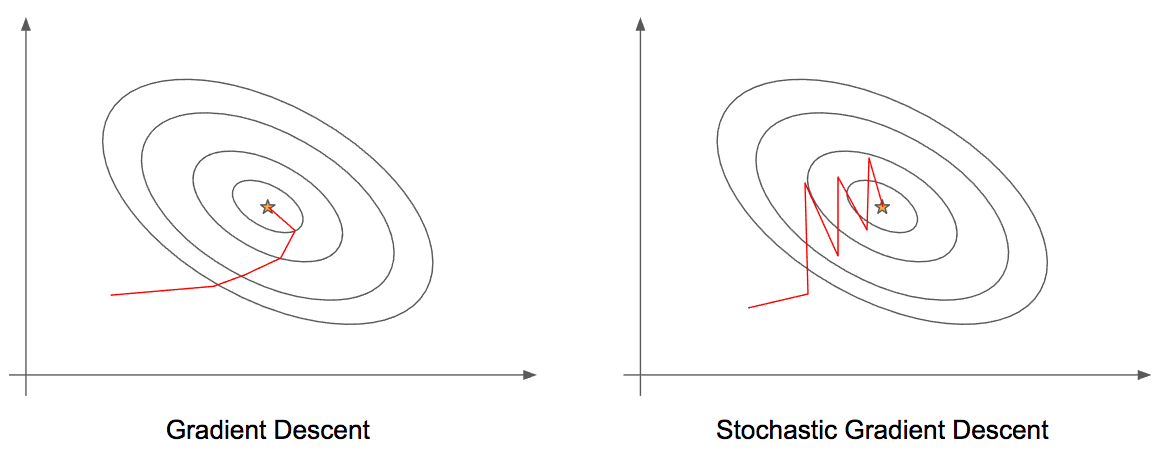
\includegraphics[width=.8\linewidth, scale=0.7]{img/figures/gradient.png}
			\caption{The different trajectories from GD and SGD.}
			\label{fig:gradient}
		\end{figure}
		%Due to its stochastic nature, c. However, it has been shown that SGD almost surely converges to the global cost minimum if the cost function is convex (or pseudo-convex)[1] [1] Bottou, Léon (1998). "Online Algorithms and Stochastic Approximations". Online Learning and Neural Networks. Cambridge University Press. ISBN 978-0-521-65263-6

		For what concernes the convergence of the stochastic gradient descent algorithm, it depends on the choice of $\eta$: it is necessary to gradually decrease the learning rate over the epochs for ensure convergence.
%deeplearning
		A sufficient condition to guarantee convergence of SGD is that the sequence of decreasing learning rates satisfy:

		\begin{equation}
			\label{delta}
			\sum_{t=1}^\infty \eta_t = \infty \text{  } \text{ and }\text{  } \sum_{t=1}^\infty \eta_t^2 < \infty
		\end{equation}

		%The cost function C(w) is three times differentiable with continuous derivatives.4 It is bounded from below, i.e. C(w) ≥ Cmin. We can assume, without loss of generality, that C(w) ≥ 0 - Online Learning and Stochastic Approximations, Leon Bottou
		Futhermore, if we assume that the Hessian matrix of the Loss function is strictly positive definite at the optimum, which means that the Loss function is strogly convex, the convergence rate is $O(\frac{1}{k})$, with \textit{k} as the number of epochs in the training. %strongly convex
		Otherwise, relaxing this assumption in presence of a convex problem, the convergence rate becomes $O(\frac{1}{\sqrt[]{k}})$\cite{Goodfellow-et-al-2016,Montavon:2012:NNT:2480981,Saad:1999:OLN:304710}.

		Unfortunatly, as we showed in \S\ref{sub:properties_of_the_loss_function}, our objective function is not convex, so we can't rely on what has been written before. Anyway, this issue seems to be overcomed: as proved in \cite{1606.04838}, the SGD is convergent even in presence of nonconvex functions.
		If the algorithm is run with a stepsize sequence satisfying Eq.\ref{delta} and the following assumptions hold:

		\begin{asu} - \label{as:conv}
  				If the level set $\mathcal{L} = \{w : \textit{L}(\textbf{W}) \leq L(\textbf{W}_1)\}$ is bounded,
  				in some neighborhood $\mathcal{N}$ of $\mathcal{L}$ the objective function \textit{L} is
  				continuously differentiable, and its gradient is Lipschitz continuous, there exist a constant $B >
  				0$ s.t. $\|\nabla\textit{L}(\textbf{W})-\nabla\textit{L}(\widetilde{\textbf{W}})\| \leq B\|
  				\textbf{W}-\widetilde{\textbf{W}}\| , \forall \textbf{W},\widetilde{\textbf{W}} \in \mathcal{N}$ ;
		\end{asu}

		\begin{asu} - \label{as:sgd_conv2}
				The Loss function \textit{L} and SGD satisfy:

				\begin{itemize}
					\item The sequence of weights ${\textbf{W}_k}$ is contained in an open set over which \textit{L} is bounded below by a scalar value $\textit{L}_{inf}$, that means the function is bounded below over the region explored by the algorithm;
					\item There exist scalars $\mu_G \geq \mu > 0 $ s.t., $\forall k \in \mathbb{N}$,
						\begin{equation}
							\nabla\textit{L}(\textbf{W}_k)^T\mathbb{E}_{\xi_k}[\textbf{g}(\textbf{W}_k,\xi_k)] \geq \mu \|\nabla\textit{L}(\textbf{W}_k)\|^2 \text{ and }
						\end{equation}
						\begin{equation}
							\|\mathbb{E}_{\xi_k}[\textbf{g}(\textbf{W}_k,\xi_k)]\|\leq \mu_G \|\nabla\textit{L}(\textbf{W}_k)\|,
						\end{equation}
						that means the vector \textbf{−g} (the extimate of the real gradient vector) is a direction of sufficient descent for \textit{L} with a norm comparable to the norm of the gradient;
					\item There exist scalars $M \geq 0 $ and $M_G \geq 0 $ s.t.:
						\begin{equation}
							\|\mathbb{V}_{\xi_k}[\textbf{g}(\textbf{W}_k,\xi_k)]\|\leq M + M_G\nabla\textit{L}(\textbf{W}_k)\|^2, \forall  k \in \mathbb{N},
						\end{equation}
						that restricts the variance of \textbf{g}.
				\end{itemize}

		\end{asu}

		then the following property is garanteed:

			\begin{equation*}
			     \lim_{k\to\infty}\mathbb{E}[\|\nabla\textit{L}(\textbf{W}_k)\|^2] = 0
			\end{equation*}

		that is the convergence of the algorithm.

		As we introduced in section \ref{sec:the_activation_functions}, each one of the units of our ANN uses the
		sigmoid function as activation function. This function bounds every layer's output in the range $(0, 1)$.
		In section \ref{sec:the_loss_function}, we have proved that our loss function is both Lipschitz continuous
		and differentiable. We can conclude that assumption \ref{as:conv} is respected. The first requirement of
		assumption \ref{as:sgd_conv2} is respected, being $L$ bounded in the interval $(0, 1)$, that is, having
		$L_{\mathit{inf}}$ eguals to $0$.

		A property of SGD is that the computation time per update does not grow with the number of training
		examples, allowing convergence even in presence of a large dataset.

		\begin{algorithm}[H]
			\caption{Stochastic Gradient Descent Algorithm. The learning rate $\eta$, the $\alpha$ term and the maximum number of epochs are given.}
			\label{alg:sgd}
			\begin{algorithmic}[1]
				\Procedure{Stochastic Gradient Descent}{}
					\State Initialize \textbf{W} and \textbf{v}
					\State $k \gets 0$
					\While {$k < max\_epochs$}
						\State Sample a minibatch of \textit{m} training examples \{\textit{$(x_0,y_0),(x_1,y_1),...,(x_m,y_m)$}\}
						\If {Nesterov Momentum}
							\State $\textbf{W} \gets \textbf{W} + \alpha \textbf{v}$
						\EndIf
						\State Compute gradient estimate: $\textbf{g} \gets \frac {1}{m} \nabla \sum_i\textit{L}(\textbf{W})$
						\State Compute velocity update: $\textbf{v} \gets \alpha \textbf{v} - \eta \textbf{g}$
						\State Apply update: $\textbf{W} \gets \textbf{W} + \textbf{v}$
					\EndWhile
				\EndProcedure
			\end{algorithmic}
		\end{algorithm}


		\subsection{Momentum}
		\label{sec:momentum}
			When computing the adjustment of the synaptic weights $\Delta\textbf{W}$ as in Eq. \ref{delta}, the choice of the learning rate $\eta$ influences the convergence of the SGD algorithm.
			The smaller is $\eta$, the smaller will be the changes in the matrix of weights and the rate of learning, but the smoother will be the trajectory.

			On the contrary, a bigger $\eta$ will bring to a faster convergence, but also to an oscillatory behaviour.

			A way to accelerate the SGD is the use of the \textit{Classical Momentum} (CM), a first order optimization technique which accelerate gradient descent, and so the learning rate of the final training.

			It consists in the adjustment of the new weigths through a velocity vector \textbf{v} that accumulates the gradient elements in the directions of reduction of the Loss function, and in a momentum coefficient $\alpha \in [0,1]$: the larger is  $\alpha$, the more the previous gradients affect the current direction.

			In this case, the classical momentum is given by:

			\begin{equation}
				\label{classical_momentum}
				\textbf{v}_k = \alpha\textbf{v}_{k-1} + \eta\nabla\textit{L}(\textbf{W}_k).
			\end{equation}

			The new synaptic weights are then updated as:
			\begin{equation}
				\label{update_momentum}
				\textbf{W}_k = \textbf{W}_{k-1}  + \textbf{v}_k.
			\end{equation}

			A variant of the CM algorithm, is the \textit{Nesterov's Accelerated Gradient} (NAG), which allows to avoid the oscillatory behaviour in the trajectory computed with CM, as visible in Fig.\ref{fig:momentum_graph}%fig2 on the importance}.

			The velocity vector \textbf{v} is computed as:

			\begin{equation}
				\label{nesterov_momentum}
				\textbf{v}_k = \alpha\textbf{v}_{k-1} + \eta\nabla\textit{L}(\textbf{W}_k + \alpha\textbf{v}_{k-1}).
			\end{equation}

			The update of the weights \textbf{W} follows the one described in Eq. \ref{update_momentum}.

			The variant respect Eq. \ref{classical_momentum}, shown in Fig.\ref{fig:momentum}, is given by the fact that the gradient $\nabla\textit{L}$ is evaluated after the current velocity is applied: NAG first update the $\textbf{W}_k$, making a jump in the direction of the previous accumulated gradient, and then evaluate the gradient in that point and makes a correction. This procedure allows it to change velocity vector $\textbf{v}_{k}$ in a faster way.

			We now discuss the convergence of a SGD using both classic momentum or Nesterov's accelerated
			gradient by providing some of the results illustrated in \cite{unified_convergence}, in particular
			the ones describing the case of the optimization of a non-convex function, that is, our case.
			We denote by $\mathbb{E}[\cdot]$ the expected value taken with respect to the distribution of the
			random variable whose observed value represents the choice of a particular minibatch at step $k$ and by
			$\mathbf{g}^{(k)}$ the estimate of the true full-batch gradient $\nabla F(\theta^{(k)})$ .

			\begin{theorem}[Convergence of Gradient Methods for Non-Convex Functions]
				Suppose $F$ is a function with $L$-Lipschitz continuous gradient,
				$\mathbb{E} \left [ || \mathbf{g}^{(i)} - \nabla F(\theta^{(i)}) ||^2 \right ] \le \delta^2$, and
				$|| \nabla F(\theta^{(i)}) || \le G$ for any $\theta^{(i)} \in \Theta$. Then, for any constant
				$C > 0$, running for k iteration the stochastic gradient method

				\begin{enumerate}
					\item with step size $\eta = \text{min} \left \{ 1\slash(2L),\ C\slash\sqrt{k + 1} \right \}$
					yields
					\begin{equation*}
					    \text{min}_{i = 0, \ldots, k} \mathbb{E} \left [ || \nabla F(\theta^{(i)}) ||^2 \right ]
					    \le \frac{2(F(\theta^{(0)})) - F^{*}}{k + 1} \text{max} \left\{ 2L,\
					    \frac{\sqrt{k + 1}}{C} \right\} + \frac{CL\delta^2}{\sqrt{k + 1}} \ and
					\end{equation*}
					\item with step size $\eta = \text{min} \left \{ (1 - \alpha)\slash(2L),\
					C\slash\sqrt{k + 1} \right \}$ and a momentum $\alpha \in [0, 1)$ yelds
					\begin{align*}
						&\text{min}_{i = 0, \ldots, k} \mathbb{E} \left [ || \nabla F(\theta^{(i)}) ||^2 \right ]
						\le \frac{2(F(\theta^{(0)}) - F^{*})(1 - \alpha)}{k + 1}
						\text{max} \left\{ \frac{2L}{1 - \alpha},\ \frac{\sqrt{k + 1}}{C} \right\} + \\
						&\frac{C}{sqrt{k + 1}}\frac{L\alpha^2 + L\delta^2(1 - \alpha)^2}{(1 - \alpha)^3}
					\end{align*}
				\end{enumerate}
				\label{theorem_1}
			\end{theorem}

			Theorem \ref{theorem_1} ensures that SGD with or without momentum converges in expectation for
			non-convex functions.

			It's worth to underline that, in case of batch mode and convex functions, Nesterov momentum brings the rate of convergence from $O(\frac{1}{k})$ (after k steps) to $O(\frac{1}{k^2})$\cite{10029946121}. % Nesterov, Y. (1983) A Method for Solving a Convex Programming Problem with Convergence Rate O(1/K2) . Soviet Mathematics Doklady, 27, 372-367.
			\begin{figure}
			\centering
				\begin{subfigure}[b]{0.4\textwidth}
					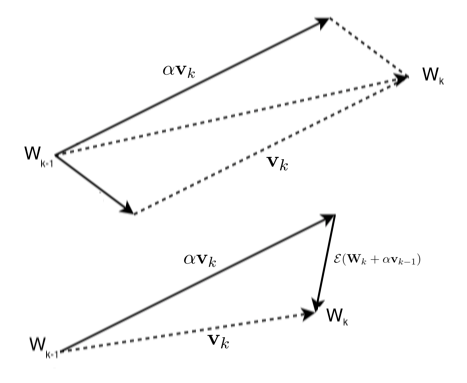
\includegraphics[width=\textwidth]{img/figures/momentum}
			  		\caption{The classical momentum on top and the Nesterov Accelerated gradient on bottom.}
				\label{fig:momentum}
				\end{subfigure}
				\qquad
				\begin{subfigure}[b]{0.4\textwidth}
					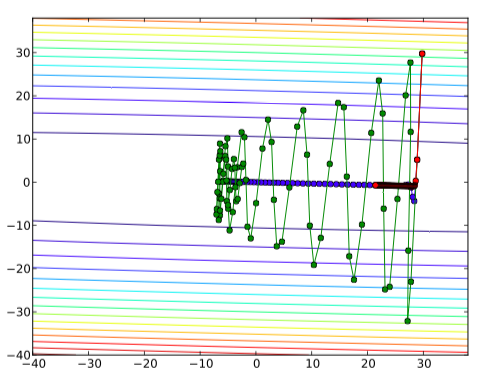
\includegraphics[width=\textwidth]{img/figures/momentum_graph}
				    \caption{The trajectory from CM (in green) and the one from NAG (in blue).}
				\label{fig:momentum_graph}
				\end{subfigure}
			\end{figure}


		\subsection{Regularization}
		\label{sec:regularization}

			In order to garantee a tradeoff between goodness and complexity of the model, the regularization is allowed in the network. This choice is important to ensure that the model doesn't grow too much in complexity.

			Regularization, in fact, adds a penalty as the model's complexity increases, forcing some weights to take values close to zero,  if they have little influence on the newtork performance and so resulting in poor generalization.

			It basically modifies the objective Loss functions as follows:

			\begin{mini}
				{\mathbf{W} \in \mathbb{R}^n} {\ \mathit{L}(\mathbf{W}) + \lambda\Omega(\mathbf{W})}{}{}
				\label{eq:reg}
			\end{mini}
			where $\Omega(\textbf{W})$ is a complexity penalty term based of the weights, and $\lambda$ is a parameter which tells how much importance must have the complexity penalty term.

			Two kinds of regularization are tipically used:

			\begin{itemize}
				\item \textit{L1}: also called Lasso Regression, which results in $\Omega(\textbf{W}) = \sum_{i=1}^{k} |w_i| = \|\textbf{W}\|_1$;
				\item \textit{L2}: also known as Ridge Regression, which results in $\Omega(\textbf{W}) = \sum_{i=1}^{k}w_i^2 = \|\textbf{W}\|_2^2$.
			\end{itemize}

			The addition of squared terms to the Loss function of Eq.\ref{mse} in the Ridge Regression, returns again a smooth continous and differentiable function. %Stochastic Gradient Descent and Regularization - Stanford CS Theory.Tim Roughgarden  Gregory Valiant

			However, the Lasso penalty, which pushes several elements of \textbf{W} to be exactly zero, making the result a sparse parameter vector, is not differentiable. So, since when applied to the Loss function, it returns a non-smooth function, it hasn't been tested on SGD\cite{journals/jmlr/Shalev-ShwartzT11}.

	\section{Nonlinear Conjugate Gradient}
	\label{sec:nonlinear_conjugate_gradient}

		An intresting optimization ables to lead to an improvement of the performances of the neural network, is the use of high-order information during the training phase: this brings to a more accurate choice of the search direction and of the step size, by using information from the second order approximation.

		In order to avoid the expensive computation of the inverse of the Hessian, we can use the \textit{Conjugate Gradient} methods, which are a class of iterative second-order optimization methods, derived from the steepest-descent algorithm, that ensure low memory requirements.

		In this way, the adjustment to the synaptic weights of the network is computed as:
		 \begin{equation}
		 	\label{weight}
		    \Delta\textbf{W} = \alpha\textbf{d},
		 \end{equation}
		where $\alpha$ is the learning rate and \textbf{d} is the new direction found.

		In our case, the nonlinear conjugate gradient methods are designed to solve the minimization problem defined in Eq.\ref{minimization}.

		As showed in the pseudocode \ref{alg:cgd}, the iterative formula generates a sequence of weights $\{W_k\}$, for every epoch of training \textit{k}, as:

		\begin{equation}
			\textbf{W}_{k+1} = \textbf{W}_{k} + \alpha_k\textbf{d}_k, \text{  }\text{  }\text{  } \textit{k} = 0,1,...,
		\end{equation}

		where $\alpha_k$ is a learning rate and $\textbf{d}_k$ is a descent direction. These are the new synaptic weights computed with the adjustment of Eq.\ref{weight}.

		% Because the error function E(~,) is nonquadratic, the algorithm will not necessarily con- verge in N steps. If the algorithm has not converged after N steps, the algorithm is restarted, i.e., initializing fik+J to the current steepest descent direction ~k+~  A Scaled Conjugate Gradient Algorithm for Fast Supervised Learning p4

		\begin{algorithm}[H]
			\caption{Nonlinear Conjugate Gradient Algorithm. The maximum number of epochs and the tolerance are given.}
			\label{alg:cgd}
			\begin{algorithmic}[1]
				\Procedure{Nonlinear Conjugate Gradient}{}
					\State Initialize $\textbf{W}_0$ and $\textit{L}_g$
					\State $k \gets 0$, $g_0 \gets 0$
					\While {$k < max\_epochs$}
						\State Evaluate the Loss function $\textit{L}_k$ and its gradient $\textbf{g}_k$
						\If {$\textit{L}_k < \textit{L}_g \text{ } \text{ or } \text{ } \|\textbf{g}_k\|> tolerance$}
							\State
							\Return Error goal reached
						\EndIf
						\State Compute the $\beta$ with one of the methods HS, MHS, FR, PR

						\State Compute the direction: $\textbf{d}_k \gets - \textbf{g}_k + \beta\textbf{d}_k$
						\State Compute the learning rate $\alpha_k$ with a Line Search
						\State Update the weights: $\textbf{W}_{k+1} \gets \textbf{W}_{k} + \alpha_k\textbf{d}_k$
						\State $k \gets k + 1$
					\EndWhile
				\EndProcedure
			\end{algorithmic}
		\end{algorithm}


		\subsection{Search Direction}
		\label{sub:search_direction}
			The direction $\textbf{d}_k$ holds the sequent property:
			\begin{equation}
			\textbf{d}_k^T\textbf{H}\textbf{d}_{tk-1} = 0,
			\end{equation}

		 	that means it is conjugate to the previous direction $\textbf{d}_{k-1}$. Furthermore, it doesn't need to know all the 	previous directions, but it only needs the last one, which is why it requires very little storage and computation.

			When dealing with quadratic functions, this method keeps the progress obtained so far in the minimization of the Loss function, by ensuring that the gradient along the previous direction does not increase.
			Anyway, it's worth to underline that this method can also be applyed with nonlinear functions: in this case, it should be necessary to restart the process, since there is no assumption that the conjugate directions previously found are still at the minimum of the function.

			Each new direction it's a linear combination of the steepest descent -\textbf{g} and the previous direction $\textbf{d}_{k-1}$, and it is defined as:
			\begin{equation}
			\label{dir}
			  \textbf{d}_k=\begin{cases}
			    -\textbf{g}_0, & \text{if $k=0$};\\
			    -\textbf{g}_k + \beta_k\textbf{d}_{k-1}, & \text{otherwise,}
			  \end{cases}
			\end{equation}

			where $\beta_k$ is a scalar, to be determined, that says how much of the previous direction should be added to the newest one. When applied to minimize a strictly convex quadratic function, it ensure that the directions $\textbf{d}_{k}$ and $\textbf{d}_{k-1}$ are conjugate with respective to the Hessian of the objective function, that is the property \ref{sub:search_direction} holds.

			Of course, the first search direction when $k = 0$ is defined as the steepest descent direction at the initial weight $\textbf{W}_0$ while, for $k > 1$, a minimization along each of the search direction is performed.

			Since it may be that the direction found is not a descent direction of the objective function, another modified search direction, proposed by Zang et al.\cite{L-2006}, has been tested in the project. It ensures sufficient descent $g_k^T = -\|g_k\|^2$, indipendent of the line search used or the convexity of the objective function, and is defined as follows:

			\begin{equation}
			\label{mod_dir}
				\textbf{d}_k^+=\begin{cases}
			    -\textbf{g}_0, & \text{if $k=0$};\\
			    -(1 + \beta_k\frac{\textbf{g}_k^T\textbf{d}_{k}}{\|\textbf{g}_k\|})\textbf{g}_k + \beta_k\textbf{d}_{k-1}^+, & \text{otherwise.}
			  \end{cases}
			\end{equation}



		\subsection{Beta}
		\label{sub:beta}
			What really makes the difference in the computation of the conjugate gradient algorithm, is the choice of the method used to compute the $\beta$ coefficient.

			In fact, there has been proposed various choices for computing it, each one giving different efficiency and properties.

			The formulas tested in our implementation are three: the Polak-Ribierère (PR), the Hestenes-Stiefel (HS) and a Modified Hestenes-Stiefel ($MHS^+$).

			One of the properties that must be garanteed, is the global convergence of the method. When the function to be minimized is convex and quadratic, indeed, the Conjugate Gradient algorithm ensures the convergence and the detection of the global minimum in at most N iterations, that is the number of dimensions. Often, expecially when N is very large, there are great chances that the algorithm terminates in less than N epochs.
			\cite{DIXON-1975}.
			However, since in our network we are dealing with a nonquadratic Loss function, as showed in \S\ref{sub:properties_of_the_loss_function}, the direction computed as in Eq. \ref{dir} could not be a descent direction. In order to avoid this issue, all the methods have been modified as follows, ensuring the global convergence \cite{doi:10.1137/0802003}:
			\begin{equation}
			\label{beta_max}
				 \beta^+ = max\{\beta, 0\}.
			\end{equation}

			This change provides a sort of restart of the algorithm, in case the $\beta$ found is negative. This is equivalent to forget the last search direction and start again the search from the steepest descent direction. The use of $\beta$ in Eq. \ref{beta_max} is similar to adopt the strategy of restarting the algorithm after N steps, initializing $d_k$ to the current steepest descent direction
			\cite{MOLLER1993525,Gilbert-1992}.

			\begin{equation}
			\label{betas}
				 \beta^{PR}_k = \frac{\textbf{g}_k^T(\textbf{g}_k-\textbf{g}_{k-1})}{\|\textbf{g}_{k-1}\|^2}, \text{ }
 				 %\beta^{FR}_k = \frac{\|\textbf{g}_{k}\|^2}{\|\textbf{g}_{k-1}\|^2}, \text{ }
 				 \beta^{HS}_k = \frac{\textbf{g}_k^T(\textbf{g}_k-\textbf{g}_{k-1})}{(\textbf{g}_k-\textbf{g}_{k-1}^T\textbf{d}_{k-1})}.
			\end{equation}

			%Powell [Griffiths-1984] was able to show that the Polak-Ribire method with exact line searches can cycle infinitely without approaching a solution point. The same result applies to the Hestenes-Stiefel method, since the two methods are identical when (gk,dk-1) 0, which holds when line searches are exact
			The HS and the PR methods in Eq. \ref{betas} have very similar performances and they are two of the most efficient conjugate gradient methods, but they are not globally convergent for nonlinear function\cite{Griffiths-1984}. That's why the modification of Eq. \ref{beta_max} has been adopted\cite{Powell-1986}, since it enforces the descent property of the algorithm.
			Both the methods are formulated in such a way that, when occurring small steps, the search direction found is close to the negative gradient direction, getting a final step of decent size\cite{Gilbert-1992}.
			Moreover, the HS method is considered superior to other methods when applied to nonquadratic functions.

			If we assume the Assumption \ref{as:conv} and we use a $\beta$ HS or PR, modified as in Eq.\ref{beta_max} and a Line Search as the one described in \S\ref{sub:line_search}, then it holds the convergence of the algorithm as follows\cite{Gilbert-1992}:

			\begin{equation}
			\label{conv_cg}
			  \lim_{k \to \infty} \|\textbf{g}_k\| = 0,
			\end{equation}
			a weaker result with respect to the one involved with strongly convex functions, $\lim_{k \to \infty} \textbf{g}_k = 0.$
			%SupposethatAssumptions2.1hold. Considerthemethod(1.2)- (1.3) with/3k max{/3R,0}, and with a line search satisfying the Wolfe conditions (2.4)-(2.5) and the sufficient descent condition (4.1). Then liminf Ilgkll O.


			%For what concernes the FR method (also described in Eq.\ref{betas}), it requires a constrain on the parameters of the inexact line search procedure of section \ref{sub:line_search}, used to identify the right step length $\alpha$. In particular, it requires that $\sigma_1 < \sigma_2 < 0.5$ in order to garantee that the Armijo Wolfe conditions are satisfied, and it seems to be less efficient and robust than the other methods \cite{Boyd:2004:CO:993483}, chapter 5.
			%Anyway, by imposing this condition, the FR method is globally convergent even when dealing with nonlinear functions.

			The last method tested is the $MHS^+$, a modified version of the Hestenes-Stiefel one \cite{LIVIERIS2013491}.
			It garantees sufficient descent with inexact line search and is based on a modified secant equation which approximates the second order information of the Loss function with high order accuracy. Moreover, it is globally convergent.

			It is defined as follows:

			\begin{equation}
			\label{mhs}
 				 \beta^{MHS}_k = \frac{\mathbf{g}_k^T \widetilde{\textbf{y}}_{k-1}^*}{\mathbf{d}_{k-1}^T\widetilde{\textbf{y}}_{k-1}^*}.
			\end{equation}

			In order to better understand the formula \ref{mhs}, it's important to describe all the components involved in its definiton.

			When dealing with quasi-Newton methods, an approximation $\textbf{B}_{k-1}$ of the Hessian of the Loss function $\nabla^2\textit{L}_{k-1}$ is update such that $\textbf{B}_k$ satisfies the secant condition:

			\begin{equation}
			\label{secant_1}
 				\textbf{B}_k (\textbf{W}_k - \textbf{W}_{k-1}) = \textbf{y}_{k-1},
 			\end{equation}

 			where $\textbf{y}_{k-1}$ is defined as $\textbf{g}_k - \textbf{g}_{k-1}$.
%new quasi newton method for unconstrain-wei

 			Wei et al. \cite{Zengxi-2006} derived a class of modified secant condition:

			\begin{equation}
			\label{secant_2}
 				\textbf{B}_{k-1} (\textbf{W}_k - \textbf{W}_{k-1}) = \widetilde{\textbf{y}}_{k-1},
 			\end{equation}


			\begin{equation}
			\label{secant_2}
 			 \widetilde{\textbf{y}}_{k-1} =  \textbf{y}_{k-1} + \frac{\theta_{k-1}}{(\textbf{W}_k - \textbf{W}_{k-1})^T\textbf{u}}\textbf{u},
 			\end{equation}

 			with \textbf{u} a vector satisying $(\textbf{W}_k - \textbf{W}_{k-1})^T\textbf{u} \neq 0$ and $\theta_{k-1}$ defined as:
 			\begin{equation}
			\label{theta}
 			 \theta_{k-1} = 2(\textit{L}_{k-1} - \textit{L}_{k}) + (\textbf{g}_k + \textbf{g}_{k-1})^T(\textbf{W}_k - \textbf{W}_{k-1}).
 			\end{equation}


 			Since for $\|(\textbf{W}_k - \textbf{W}_{k-1})\| > 1$ the standard secant Eq.\ref{secant_1} better approximates $\nabla^2\textit{L}_{k-1}(\textbf{W}_k - \textbf{W}_{k-1})$ than the modified version in Eq.\ref{secant_2}, Livieris and Pintelas\cite{LIVIERIS2013491} proposed a modification of the equation in this way:

 			\begin{equation}
			\label{secant_3}
 				\textbf{B}_{k-1} (\textbf{W}_k - \textbf{W}_{k-1}) = \widetilde{\textbf{y}}_{k-1}^*,
 			\end{equation}

 			\begin{equation}
			\label{y_3}
 				\widetilde{\textbf{y}}_{k-1}^* = \textbf{y}_{k-1} + \rho_{k-1} \frac{max\{\theta_{k-1},0\}}{(\textbf{W}_k - \textbf{W}_{k-1})^T\textbf{u}}\textbf{u},
 			\end{equation}

 			where $\rho_{k-1} \in \{0,1\}$ is a parameter that switch between the standard secant equation Eq.\ref{secant_1} and the modified one Eq.\ref{secant_3}, setting $\rho_{k-1}$ as:

			\begin{equation}
			\label{rho}
			  \rho_{k-1} =\begin{cases}
			    1 , & \text{if }\|(\textbf{W}_k - \textbf{W}_{k-1})\| \leq 1;\\
			    0 , & \text{otherwise.}
			  \end{cases}
			\end{equation}

			Since the following assumptions are satisfied by the Loss functions in Eq.\ref{mse}:

			\begin{asu} - \label{as:1}
  				The level set $\mathcal{L} = \{w \in \mathbb{R}^n | \textit{L}(\textbf{W}) \leq L(\textbf{W}_0)\}$ is bounded, there exist a constant $B > 0$ s.t. $\|\textbf{W}\| \leq B, \forall \textbf{W} \in \mathcal{L}$;
			\end{asu}

			\begin{asu} - \label{as:2}
				If in some neighborhood $\mathcal{N} \in \mathcal{L}$, \textit{L} is differentiable and its gradient \textbf{g} is Lipschitz continuous, then there exists a constant $ L > 0 $ such that
				\begin{equation}
				\label{ass2}
				  \|\textbf{g}(\textbf{W})-\textbf{g}(\widetilde{\textbf{W}})\|, \forall \textbf{ W},\widetilde{\textbf{W}} \in \mathcal{N},
				\end{equation}
			\end{asu}
			if the conjugate gradient algorithm is performed using $MSH^+$ and computing the search direction $\textbf{d}^+$ as defined by Eq.\ref{mod_dir}, we have:

			\begin{equation}
			\label{conv_mhs}
			  \lim_{k \to \infty} \|\textbf{g}_k\| = 0,
			\end{equation}

			that is the convergence of the algorithm.

			Assumption \ref{as:1} is satisfied, since, as we have said before, our loss function is bounded in the
			interval $(0, 1)$, and hence the level set is also bounded. Assumption \ref{as:2} is also satisfied,
			having described the properties for our loss function in section \ref{sec:the_loss_function}.

		\subsection{Line Search}
		\label{sub:line_search}
			Once computed the new direction \textbf{d} involved in the new weights \textbf{W}+$\alpha$\textbf{d}, a line search has to be implemented in order to find the right step size which minimize the Loss function.

			The step size $\alpha$ is nothing more than a scalar: the learning rate for the conjugate gradient algorithm, which tells how far is right to move along a given direction.

			So, fixed the values of the weights \textbf{W} and the descent direction \textbf{d}, the main goal is to find the right value for $\alpha$ that is able to minimize the Loss function:

			 \begin{mini}
			   {\alpha}{\textit{L}(\textbf{W} + \alpha\textbf{d}).}{}{}
			 \end{mini}

			Of course, we have to deal with a tradeoff: we want a good reduction, but we can't spend too much time computing the exact value for the optimum solution. So, the smarter way to get it is to use an inexact line search, that try some candidate step size and accepts the first one satisfying some conditions.

			This search is performed in two phases:
			\begin{itemize}
			\item a \textit{bracketing phase}, that finds an initial interval containing a minimizer;
			\item an \textit{interpolation phase} that, given the interval, finds the right step length in it.
			\end{itemize}

			We decided to use one of the most popular line search condition: the \textit{Armijo-Wolfe} condition.

			The search for the better $\alpha$ is led by two condition:
			\begin{itemize}
			\item the \textit{Armijo} one:
			\begin{equation}
			\textit{L}(\textbf{W}_k+\alpha _k\textbf{d}_k)\leq \textit{L}(\textbf{W}_k)+\sigma_1\alpha\nabla \textit{L}_k^T\textbf{d}_k
			\end{equation}

			which ensure that $\alpha$ gives a sufficient decrease of the objective function, being this reduction proportional to the step length $\alpha$ and the directional derivative $\nabla \textit{L}_k^Td_k$.

			The constant $\sigma_1$ has been set $\sigma_1=10^{-4}$, since it is suggested in literature to be quite small.

			\item the \textit{Strong Wolfe} condition:
			\begin{equation}
			|\nabla \textit{L}(\textbf{W}_k+\alpha _k\textbf{d}_k)^T\textbf{d}_k|\leq \textit{L}(\textbf{W}_k)+\sigma_2|\nabla \textit{L}_k^T\textbf{d}_k|
			\end{equation}
			which garantees to choose steps whose size is not too small.

			It is also known as curvature condition and ensures that, moving of a step $\alpha$ along the given direction, the slope of our function if greater than $\sigma_2$ times the original gradient (if the slope is only slightly negative, the function cannot decrease rapidly along that direction, so it's better to stop the search).

			In this case, the constant $\sigma_2$ is equal to 0.1, since a smaller value gives a more accurate line search.
			Futhermore, having choosen the strong condition, which doesn't allow the derivative to be too positive, we are sure that the $\alpha$ found lies close to a stationary point of the function.
			\end{itemize}

			\begin{algorithm}
			\caption{Line Search satisfying the strong Wolfe conditions. $\alpha_1 > 0$ and $\alpha_{max}$ are given.}\label{alg:linesearch}
			\begin{algorithmic}[1]
				\Procedure{line\_search}{}
				\State $\alpha_0 \gets \textit{0};$
				\State $i \gets \textit{1};$
				\While {$i \leq max\_iter$}
				 		\State  $ \text{Evaluate}\textit{L}(\alpha_i);$
						\If  { $[\textit{L}(\alpha_i) > \textit{L}(0) + \sigma_1\alpha_i\nabla\textit{L}_0^Td_0] \text{  or  } [\textit{L}(\alpha_i)\leq \textit{L}(\alpha_{i-1}) \text{  and  } i>1]  $ }
							\State $\alpha_* \gets \textbf{zoom}(\alpha_{i-1},\alpha_{i});$
							\Return $\alpha_*; $
						\EndIf
						\State   $\text{Evaluate } \nabla\textit{L}_{i} $
						\If  { $|\nabla\textit{L}_{i}| \leq -\sigma_2\nabla\textit{L}_0^Td_0 $}
							\State $\alpha_* \gets \alpha_i; $
							\Return $\alpha_*; $
						\EndIf
						\If  { $\nabla\textit{L}_{i} \geq 0$ }
							\State $\alpha_* \gets \textbf{zoom}(\alpha_{i},\alpha_{i-1}); $
							\Return $\alpha_*; $
						\EndIf
						\If  { $(|\textit{L}_{i} - \textit{L}_{i-1}| \leq threshold$ }
							\State $\alpha_* \gets\alpha_{i}$
							\Return $\alpha_*;$
						\EndIf
						\State $\text{Choose  } \alpha_{i+1}  \in (\alpha_i, \alpha_{max});$
						\State $i \gets i+1; $
				\EndWhile
			\EndProcedure
			\end{algorithmic}
			\end{algorithm}


			\begin{algorithm}
				\caption{Zoom}
				\label{alg:zoom}
				\begin{algorithmic}[1]
					\Procedure{Zoom}{}
						\While{True}
							\State  $ \alpha_j \gets \textit{quadratic\_interpolation}(\alpha_{lo}, \alpha_{hi}); $
							\State $ \text{Evaluate }\textit{L}(\alpha_j);$
							\If{$\left [ \textit{L}(\alpha_j) > \textit{L}(0) + \sigma_1 \alpha_j
							    \nabla  \textit{L}_0^T d_0 \right ]$ or $\left [ \textit{L}(\alpha_j) \leq
							    \textit{L}(\alpha_{lo}) \right ]$}
							    \State $\alpha_* \gets \alpha_j; $
								\State \Return $\alpha_*; $
							\Else
								\State $\text{Evaluate } \nabla \textit{L}_j^T d_j; $
								\If{$\left | \nabla \textit{L}_j^T d_j \right | \leq -\sigma_2 \nabla
								    \textit{L}_0^T d_0$}
								    \State $\alpha_* \gets \alpha_j; $
									\State \Return $\alpha_*; $
								\EndIf
								\If{$\nabla \textit{L}_j^T d_j (\alpha_{hi}-\alpha_{lo}) \geq 0 $}
									\State $\alpha_{hi} \gets \alpha_{lo}; $
								\EndIf
								\If{$(|\textit{L}_{j} - \textit{L}_{0}| \leq threshold$}
									\State $\alpha_* \gets\alpha_{j}$
									\State \Return $\alpha_*;$
								\EndIf
							\EndIf
						\State $\alpha_{lo} \gets \alpha_{j}; $
			{}			\EndWhile
					\EndProcedure
				\end{algorithmic}
			\end{algorithm}

			The algorithm satisfing the Strong Wolfe conditions is implemented through the functions described in the pseudocodes \ref{alg:linesearch}, \ref{alg:zoom} and is based on the the algorithms presented in \cite{Boyd:2004:CO:993483}, chapter 3.

			Since two consecutive values may be similar in finite-precision arithmetic, we set a threshold in both the \texttt{line\_search} and the quadratic interpolation functions, which garantees that the algorithm stops if two values of $\alpha$ are too close or if the maximum number of iterations has been reached.

			%The \texttt{line\_search} function try to find and return a good $\alpha$; if it fails, it returns an interval in which continue the searching, invoking the \texttt{zoom} function, which decreases the size of the interval, until it finds and returns a good step length.

			%\texttt{Zoom} invokes another function, \texttt{interpolate\_alpha}, which is nothing more than the implementation of a bisection interpolation in order to find a trial $\alpha$ inside the given interval.





			% \begin{algorithm}
			% \caption{Interpolate}\label{bisection}
			% \begin{algorithmic}[1]
			% \Procedure{interpolate\_alpha}{}
			% \State $i \gets \textit{1};$
			% \While {$i \leq max\_iter$}
			% 	\State $\alpha_{mid} \gets (\alpha_{hi}-\alpha_{lo})/2$
			% 	\State  $ \text{Evaluate }\textit{L}(\alpha_{mid});$
			%  	\If  { $[\textit{L}(\alpha_{mid}) == 0]  \text{  or  }  [(\alpha_{hi}-\alpha_{lo})/2 < threshold] $ }
			% 			\Return $\alpha_{mid}; $
			% 	\EndIf
			% 	\State   $\text{Evaluate } \textit{L}(\_{mid}alpha_{lo}); $
			% 	\If  { $sign(\textit{L}(\alpha_{mid})) == sign(\textit{L}(\alpha_{lo}))$ }
			% 		\State $\alpha_{lo} \gets \alpha_{mid}; $
			% 	\Else
			% 		\State $\alpha_{hi} \gets \alpha_{mid}; $
			% 	\EndIf
			% 	\State $i \gets i+1; $
			% \EndWhile
			% \EndProcedure
			% \end{algorithmic}
			% \end{algorithm}
